\documentclass[12pt]{article}
\usepackage[margin=1in]{geometry} 
\usepackage{amsmath,amsthm,amssymb,amsfonts, }
\usepackage{enumitem}
\usepackage{placeins}
\usepackage{mathtools, eucal}
\usepackage{graphicx}
\usepackage{color}
\usepackage{subcaption}

\usepackage{amsmath,amsgen,amstext,amsbsy,amsopn,amsfonts,amsthm}
% standard AMS packages for symbols, formats, etc.
\usepackage{graphicx,tabularx,array,geometry,float}
%\usepackage{hyperref}
% packages for web interface, graphics, etc,

 
\newtheorem{remark}{Remark}
 
\begin{document}
 
%\renewcommand{\qedsymbol}{\filledbox}
%Good resources for looking up how to do stuff:
%Binary operators: http://www.access2science.com/latex/Binary.html
%General help: http://en.wikibooks.org/wiki/LaTeX/Mathematics
%Or just google stuff
 
\title{Homework 8 Solutions}
\author{Fangroup}
\maketitle

\section*{Problem 4 (5.1)}

\begin{figure}[htbp]
  \caption{Figures of all functions}
  \centering
    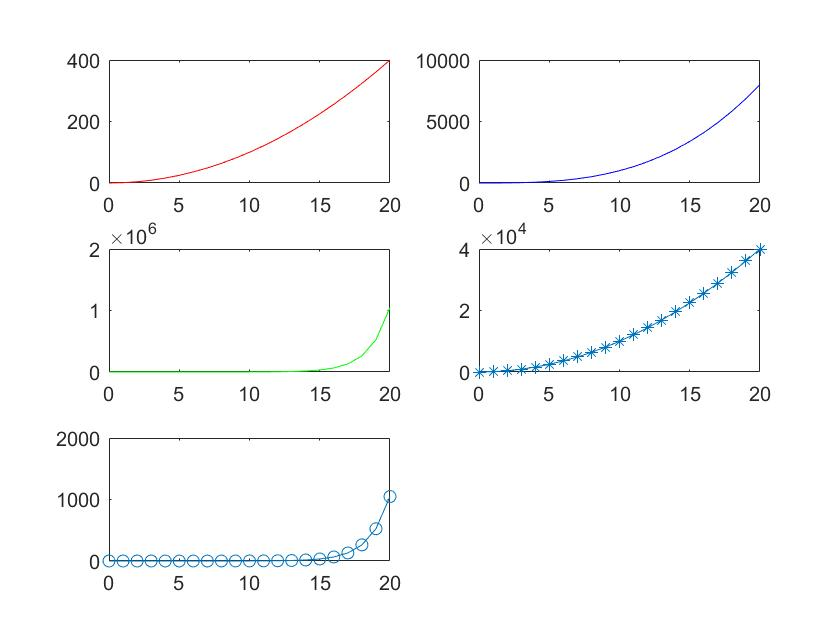
\includegraphics[width=0.5\textwidth]{Fig1.jpg}
    \label{fig1}
\end{figure}


\begin{enumerate}
\item [(a)]

\begin{figure}[htbp]
  \caption{Part(a)}
  \centering
    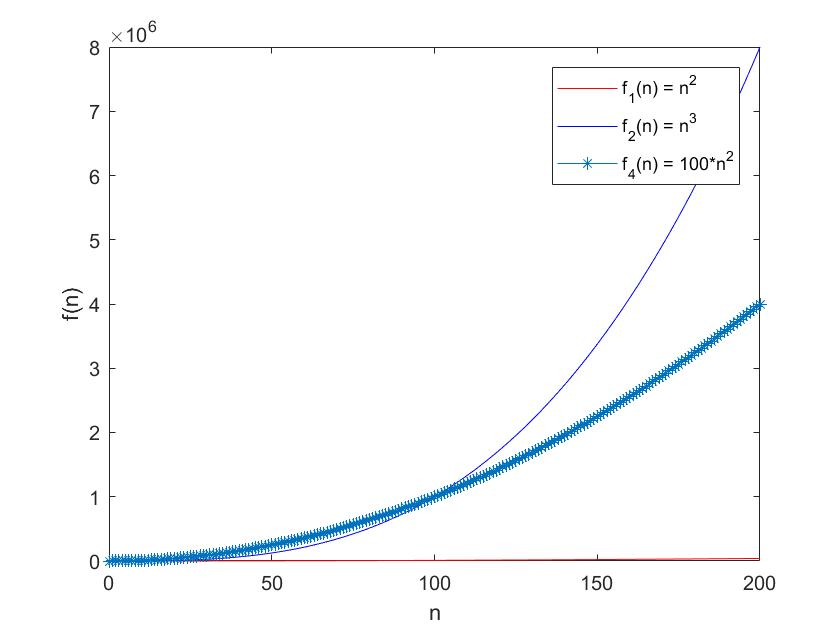
\includegraphics[width=0.5\textwidth]{part_a.jpg}
    \label{part_a}
\end{figure}

From Fig.\ref{part_a} we can see that a quadratic method does not always perform better than a cubic algorithm. It depends on the scale of the problem. $f_2$ is not always less than $f_4$.

\item [(b)]

\begin{figure}[htbp]
  \caption{Part(b)}
  \centering
    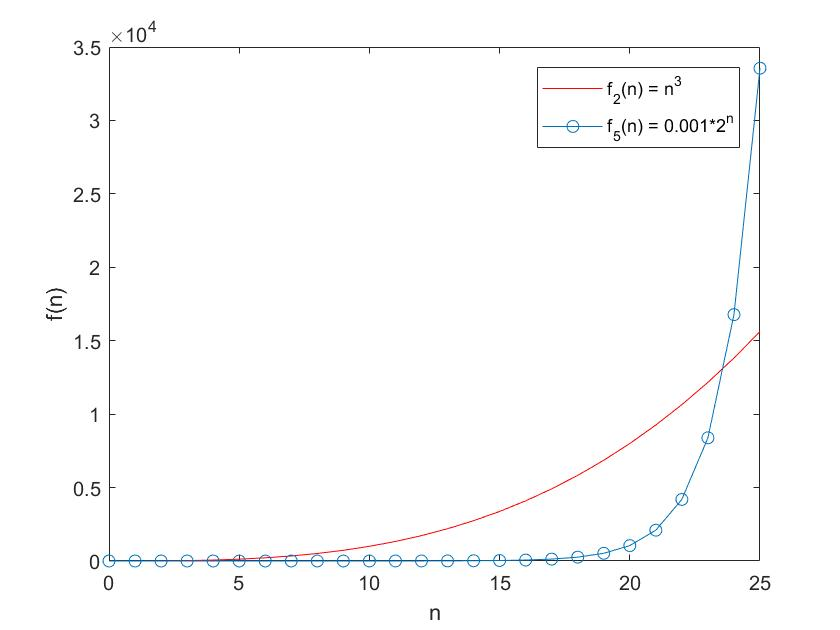
\includegraphics[width=0.5\textwidth]{part_b.jpg}
    \label{part_b}
\end{figure}

Similarly, a polynomial algorithm doesn't always perform better than exponential algorithm. $f_2$ is not always less than $f_5$.

\end{enumerate}





\section*{Problem 5 (7.1)}



(Thanks to Dr. Nie for the solution)

\begin{itemize}
	\item[(a)] W.l.o.g, we assume that the linear programming problem is in the standard form \begin{align*}
	\min ~c^Tx~\quad\text{s.t.} ~Ax=b, ~x\geq 0,
	\end{align*}where $A\in\mathbb{R}^{m\times n}$, $c\in\mathbb{R}^n$ and $b\in\mathbb{R}^m$. Given a basis $B$, the corresponding basic solution can be obtained by solving the following system of linear equations: 
	\begin{align*}
	\left( \begin{array}{ll} B & N \\ 0 & I \end{array}\right) \left( \begin{array}{l}x_B\\x_N\end{array}\right) =\left( \begin{array}{l}b\\0\end{array}\right)
	\end{align*}
	Therefore, using Algorithm A, we are able to list all the basic solutions to this LP problem. Then, the LP problem can be solved by finding the basic feasible solution with minimal objective value.
	
	\item[(b)] Given a system of linear equations, we construct a linear programming problem whose objective function is constant and feasible domain is defined by those linear equations. Using Algorithm B, we are able to solve the LP problem, i.e., obtain an optimal solution. This optimal solution is feasible, and thus solves the system of linear equations. 
	\item[(c)] From (a) and (b), it is of the same difficulty (computational complexity) to solve systems of linear equations and linear programming problems, respectively. Since the systems of linear equations can be solved in polynomial time, we know that linear programming problems are polynomial-time solvable. 
\end{itemize}


\section*{Problem 6}

\begin{proof}

\begin{enumerate}
\item [(T1)]
$\forall \textbf x^k \in int(\mathbb R^n_+)$, i.e., $x^k_i >0, \forall i = 1, \dots, n$, matrix $X_k = diag(x^k_1, \dots, x^k_n)$ is invertible. Hence, $T_k(\textbf x) \in \mathbb R^n_+$. And it is also clear that $T(\textbf x) = T(\textbf y)$ when $ \textbf x = \textbf y$.

\item [(T2)]
Straight forward algebra. 

$$
T_k(\textbf x^k) = X_k^{-1}\textbf x^k = diag(x^k_1, \dots, x_n^k) \begin{pmatrix}
x^k_1 \\ \vdots \\ x^k_n
\end{pmatrix} = 
\begin{pmatrix}
1 \\ \vdots \\ 1
\end{pmatrix} = \textbf e.
$$

\item [(T3)]
The only vertex of $\mathbb R^n_+$ is the origin. And $T(\textbf 0)= \textbf 0$.

\item [(T4)]

Suppose $\textbf x \in bdry(\mathbb R^n_+)$. Hence, $\exists i$ such that $x_i = 0$. Then, the ith element of $T(\textbf x)$, denote as $y_i$, is $y_i = x_i/x^k_i = 0$. Hence, $T(\textbf x)\in bdry(\mathbb R^n_+)$.

\item [(T5)]

Suppose $\textbf x \in int(\mathbb R^n_+)$. i.e., $\forall i, x_i > 0$. Then, for any element of $T(\textbf x)$, denote as $y_i$, we have $y_i = x_i/x^k_i > 0, \forall i$. Hence, $T(\textbf x)\in int(\mathbb R^n_+)$.

\item [(T6)]
To show $T_k$ is one-to-one, we need to show that if $\textbf x \neq \textbf y \in \mathbb R^n_+$, then $T_k(\textbf x) \neq T(\textbf y)$. Indeed, if $\textbf x \neq \textbf y$, then $\exists j$ such that $x_j \neq y_j$ and so $x_j/x^k_j \neq y_j/x^k_j$. Hence, $T_k(\textbf x) \neq T(\textbf y)$.

$T_k$ is an onto mapping. Indeed, for each $\textbf z \in \mathbb R^n_+$, we can find $\textbf x = X_k \textbf z \in \mathbb R^n_+$ such that $T_k(\textbf x) = \textbf z$. 

Hence $T_k$ is a linear bijection and so it has inverse mapping. Let $T^{-1}_k(\textbf y)= X_k\textbf x$. Then we only need to check that $T_k\circ T_k^{-1} = T_k^{-1} \circ T_k = I$. It is obvious.
 


\end{enumerate}



\end{proof}




\end{document}